\chapter{Numerical methods to simulate dispersed phase}
\label{ch3:disperse_phase_methods}

\section{Introduction}

The previous chapter presented numerical methodologies applicable to separate two-phase flows. These are useful for solving problems where the dynamics of atomization need to be accurately resolved. Nonetheless, those methods cannot be applied in the dispersed phase regime, where atomization is complete (or almost complete) and a spray composed of individual droplets is formed. Such problems, often found when studying reactive processes where fuel is injected into a combustion chamber, need a different representation of the liquid phase so that 1) the spray can be transported with acceptable computational costs and 2) can include more complex physics relevant to reactive problems, such as evaporation and combustion.

The spray generated in the dispersed phase regime is mainly distinguished from liquid in the separate regime by the following features (represented in Figure \ref{fig:atomization_regimes_herrmann}):

\begin{itemize}

	\item The characteristic length scales of the particles. In dispersed phase flows, these ones are low and usually smaller than the resolution of the main grid.
	
	\item The value of the liquid volume fraction $\alpha_l$. In dispersed phase flows, $\alpha_l < 1$. According its value, one can distinguish between dense regime (moderate values of $\alpha_l$, particles are close to each other) and dilute regime (lower values of $\alpha_l$, usually below $10^{-3}$, particles are far from each other).

\end{itemize}

The numerical formalisms to resolved dispersed phase flows will hence depend on these two characteristics. It is also important to consider the interaction with the gaseous phase, since this one will depend by the resolution of the main grid. The interaction between the liquid and gaseous phases in dispersed phase flows can be quantified by means of the Stokes number $St$, defined as the ratio between the characteristic time-scale of a liquid particle $\tau_p$ and a characteristic time of the gaseous phase $\tau_g$: 

\begin{equation}
\label{eq:Stokes_number_definition_general}
St = \frac{\tau_p}{\tau_g}
\end{equation}

A classification of numerical methods to simulate dispersed phase flows based on the volume fraction and the Stokes number has been done by \textbf{ref:2009-Balachandar}, shown in Figure \ref{fig:balachandar_numerical_methods_representation}. As it can be seen, the Stokes number will depend on the numerical methodology used to resolve the gaseous phase: in DNS, the smallest scales of turbulence with characteristic size $\upeta$ will be resolved and will have a characteristic time $\tau_k$, while in LES the smallest scales resolved $\upxi$ will be larger and their time-scales will be different ($\tau_\upxi$). Regarding the volume fraction, coupling strategies between liquid particles and gas can be used depending on its value: in the dilute regime particles are far from each other and the interactions among them can be neglected (one and two-way coupling), while in the dense regime the interaction between particles must be taken into account (four-way coupling). The difference between one and two-way coupling depends on if the influence of the liquid phase onto the gas is considered with source terms (two-way coupling) or if it is neglected, so that the gaseous phase will not be perturbed by the particles (one-way coupling).


\begin{figure}[h!]
	\centering
	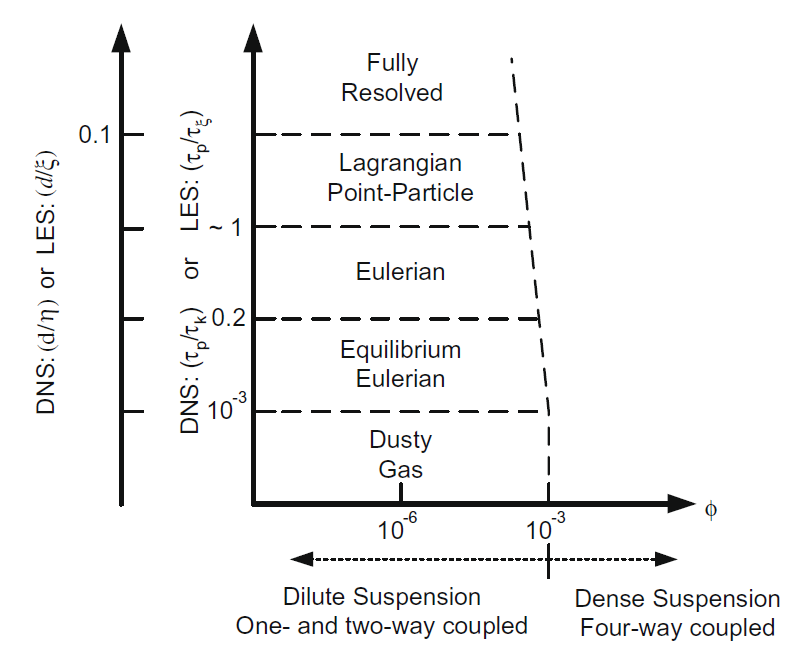
\includegraphics[scale=0.6]{./part1_numerical_approaches/figures_ch3/balachandar_disperse_phase_classification}
	\caption{Several numerical approaches to solve dispersed phase flows. Classification is done with respect to the liquid volume fraction (here defined as $\phi$) and to the Stokes number or, equivalently, to the ratio of largest to smallest length scales, which depend on the numerical resolution.  Source: \textbf{ref:2009-Balachandar}}
	\label{fig:balachandar_numerical_methods_representation}
\end{figure}


\subsection{Existing approaches to model dispersed phase flows}



Several approaches exist to study disperse phase. 

Comment statistical approaches ( 2000 SUbramanian, 2013 Vie, Vie 2013). Mention that they are out of the scope of this thesis, so we are gonna focus on EE and EL.

%\section{Spray characterisation (??)}

%Maybe this can be a subsection of the next section ?

In this chapter, 

\section{Eulerian formalisms for dispersed phase}

One common numerical method to solve

An Eulerian description of the fluid flow (EE) takes a control volume and averages the properties of the fluid flow within it. Both the carrier and dispersed phase are resolved in the same grid, which can save computational time. For characterizing the dispersed phase, averaged properties and statistical tools are used to solve the Navier-Stokes equations. It presents, however, the following disadvantages \citepColor[garcia_developpement_2009]:

\begin{enumerate}

\item A non-robust system of equations is produced.

\item Interactions of the particles with the walls and among themselves are very difficult (if not impossible) to model.

\end{enumerate}

The carrier phase is solved from the Navier-Stokes equations (\ref{eq:navier-stokes}) applied to gas, neglecting the conservation of species as there are no chemical reactions. In order to develop the equations for the disperse, the following assumptions need to be made \citepColor[lancien_etude_2018]:

\begin{enumerate}

\item The atomization process is complete: no further breakup occurs, and the particles are perfectly spherical droplets.

\item The density ratio between gas and liquid allows to assume that the only force exerted by the carrier phase on the droplets is drag.

\item The temperature, and therefore the sensible enthalpy, is assumed to be homogeneous inside each droplet.

\item A dilute spray assumption is made ($\alpha_l < 0.01$), so the liquid volume fraction is negligible before the gaseous one: $\alpha_g = 1 - \alpha_l \approx 1$. This leads to the next two hypotheses.

\item The interactions between droplets are negligible.

\item The liquid phase has little influence over the carrier phase, which allows the use of a probability density function conditioned by one realization.

\item The spray is mono-disperse and mono-kinetic: at one point in time and space, the droplets all have the same diameter and velocity.

\item Similarly, at one point in time and space, the droplets have the same temperature.

%\item Random uncorrelated motion is neglected.

\end{enumerate}

For the disperse phase, the corresponding equations are:


\begin{subequations}
\label{eq:EE_disperse_phase}
\begin{align}
\frac{\partial \breve{n}_l}{\partial t} + \frac{\partial \breve{n}_l \breve{u}_{l,i}}{\partial x_i} &= 0 \\
\frac{\partial \rho_l \breve{\alpha}_l}{\partial t} + \frac{\partial \rho_l \breve{\alpha}_l \breve{u}_{l,i}}{\partial x_i} &= - \Gamma \\
\frac{\partial \rho_l \breve{\alpha}_l \breve{u}_{l,j}}{\partial t} + \frac{\partial \rho_l \breve{\alpha}_l \breve{u}_{l,i} \breve{u}_{l,j}}{\partial x_i} &= \mathcal{T} \left( u''_{p,j} \right) - \Gamma \breve{u}_{l,j} + F_{d,j} \\
\frac{\partial \rho_l \breve{\alpha}_l \delta \breve{\theta}_l}{\partial t} + \frac{\partial \rho_l \breve{\alpha}_l \breve{u}_{l,i} \delta \breve{\theta}_l }{\partial x_i} &= \mathcal{T} \left( \frac{1}{2} u''_{p,j} u''_{p,j} \right) + \mathcal{U}_\theta - \Gamma \delta \breve{\theta}_l + W_\theta \\
\frac{\partial \rho_l \breve{\alpha}_l \breve{h}_{s,l} }{\partial t} + \frac{\partial \rho_l \breve{\alpha}_l \breve{u}_{l,i} \breve{h}_{s,l} }{\partial x_i} &= \Lambda_l + \Phi_l 
\end{align}
\end{subequations}

Details on the equations and on their terms is not given here, as the EE method will not be used in this project. A more rigorous explanation of this model can be found in \citeColor[jaegle_large_2009] and in \citeColor[lancien_etude_2018].

\section{Lagrangian point particle representation}
\label{sec:ch3_EL_formalisms}


The Lagrangian description (EL) does not use an averaging process in the grid for the fluid phase, but tracks each fluid particle individually. Every droplet is represented by its own equations which are not solved in the main grid (i.e. the Eulerian grid used to represent the carrier phase). This can make convergence difficult and hinders the introduction of parallelism techniques. However, the resulting system of equations is robust, the time per iteration is usually lower than for the EE description, and the drop-drop and drop-wall interactions are easier to model.

When considering droplets immersed in a gas, it is necessary to take into account mechanics of particle motion. A useful definition to study the relative influence between the droplet and the gas is the \textbf{Stokes number}, which is defined as the ratio between the characteristic time of the particle $\tau_p$ and the frequency of the flow fluctuations $f_{turb}$ around an obstacle \citepColor[koch_spray_2019]:

\begin{equation}
St = \tau_p f_{turb} = \frac{\tau_p \widetilde{\boldsymbol{u}}_g}{d_p}
\end{equation}

where $\widetilde{\boldsymbol{u}}_g$ is the gas velocity at the position of the particle $p$ assuming that the flow field is locally undisturbed by the presence of that particle. The Stokes number indicates how the droplet responds to fluctuations of the gas flow. If $St << 1$, the droplet will follow perfectly the fluctuations of the gas flow. On the contrary, if $St >> 1$ the droplets will rather neglect the flow trajectories and follow a ballistic trajectory. $\tau_p$ is obtained from the following expression (\textbf{CHECK THIS OUT}):


\begin{equation}
\tau_p = \frac{d_p^2 \rho_p}{18 \mu_\mathrm{g}} =  \frac{4}{3} \frac{\rho_p}{\rho_\mathrm{g}} \frac{d_p}{C_D | \boldsymbol{v}_r |} = \frac{4}{3} \frac{\rho_p d_{p^2}}{\mu_g Re C_D}
\end{equation}

For the description in the Lagrangian framework, each particle will be modelled according to the \textbf{Discrete Particle Simulations} (DPS) approach. DPS assumes each particle to be completely spherical and robust. With these assumptions, the \textbf{dynamic equations} for a particle $p$ in the spatial direction $i$ are:

\begin{subequations}
\label{eq:TPF_lagrange_dynamic_eqs}
\begin{align}
\frac{d \boldsymbol{x}_p}{d t} &= \boldsymbol{u}_p \\
\frac{d \boldsymbol{u}_p}{d t} &= \underbrace{ - \frac{3}{4} \frac{\rho_\mathrm{g}}{\rho_p} \frac{C_D}{d_p} | \boldsymbol{v}_r | \boldsymbol{v}_r }_{\text{Drag}\atop\text{term}}  + \underbrace{ \left( 1 - \frac{\rho_\mathrm{g}}{\rho_p} \right) \boldsymbol{g} }_{\text{Gravity}\atop\text{term}} 
\end{align}
\end{subequations}

% \frac{d u_{p,i}}{d t} &= \underbrace{ - \frac{3}{4} \frac{\rho_\mathrm{g}}{\rho_p} \frac{C_D}{d_p} | \boldsymbol{v}_r | v_{r,i} }_{\text{Drag}\atop\text{term}}  + \underbrace{ \left( 1 - \frac{\rho_\mathrm{g}}{\rho_p} \right) g_i }}_{\text{Gravity}\atop\text{term}} 

where $\rho_\mathrm{g}$ and $\rho_p$ are the gas and liquid particle densities respectively, $C_D$ is a drag coefficient, $d_p$ is the particle diameter, $\boldsymbol{v}_r$ is the relative velocity of the particle with respect to the airflow and $g$ is the gravity term. Equation (\ref{eq:TPF_lagrange_dynamic_eqs}b) is the momentum equation of the droplet and contains the contributions of the two forces considered: the drag force and the gravitational forces. The relative velocity is given by $\boldsymbol{v}_r = \boldsymbol{u}_p - \widetilde{\boldsymbol{u}}_g$ 

The drag coefficient $C_D$ is given by the following expression:

\begin{equation}
\label{eq:Re_CD_droplet}
C_D =
\left\{
    \begin{split}
     \frac{24}{Re} \left( 1 + 0.15 Re^{0.687} \right)\,\,\mathrm{if}\,\,Re < 1000 \\ 
    0.44\,\,\mathrm{if}\,\,Re \geq 1000 
    \end{split}
\right.
\end{equation}

where $Re = \rho_\mathrm{g} | \boldsymbol{v_r} | d_p / \mu_\mathrm{g} $. This expression was obtained experimentally by \citeColor[schiller_drag_1935] with the assumptions that the particles are perfectly spherical and rigid.  

%These assumptions also allow for the definition of the characteristic time of a particle $p$:

%\begin{equation}
%\tau_p = \frac{d_p^2 \rho_p}{18 \mu_\mathrm{g}} =  \frac{4}{3} \frac{\rho_p}{\rho_\mathrm{g}} \frac{d_p}{C_D | \boldsymbol{v_r} |} 
%\end{equation}

Besides the dynamic equations, it is also necessary to account for the \textbf{phase transition} of the liquid dispersed phase into gaseous phase. 

\begin{subequations}
\label{eq:TPF_lagrange_phasetransition_eqs}
\begin{align}
\frac{d m_p}{d t} &= \dot{m}_p = \Gamma \\
\frac{d h_p}{d t} &= \Phi_p
\end{align}
\end{subequations}

Equation (\ref{eq:TPF_lagrange_phasetransition_eqs}a) accounts for the \textbf{evaporation} process. If the uniform temperature model is used, then (\ref{eq:TPF_lagrange_phasetransition_eqs}) is equal to (\ref{eq:evaporation_mass_flow_rate}). Equation (\ref{eq:TPF_lagrange_phasetransition_eqs}b) accounts for the energy transfer. By considering the effects of the \textbf{conduction} and the \textbf{evaporation} processes in terms of energetic balance, $\Phi_p$ can be extended as follows:

\begin{equation}
\Phi_p = m_p C_{P_\mathrm{g}} \frac{d T_p}{d t} = \underbrace{ h_p \pi d_p^2 \left( T_\mathrm{g} - T_p \right) }_{\text{Conduction}\atop\text{term}} - \underbrace{ \dot{m}_p  \Delta h_v }_{\text{Evaporation}\atop\text{term}}
\end{equation}

where $C_{P_\mathrm{g}}$ is the gas specific heat capacity at constant pressure, $T_p$ is the particle temperature, $T_\mathrm{g}$ is the gas temperature, $h_p$ is the film coefficient of the gas at the particle surface and $\Delta h_v$ is the latent heat of vaporization of the particle. 

By considering Equations (\ref{eq:TPF_lagrange_dynamic_eqs}) and (\ref{eq:TPF_lagrange_phasetransition_eqs}) with all the simplifications stated, the final set of equations for the Lagrangian dispersed phase approach is:

\begin{subequations}
\begin{align}
\frac{d x_{p,i}}{d t} &= u_{p,i} \\
\frac{d u_{p,i}}{d t} &= - \frac{u_{p,i} - \widetilde{u}_{g,i} }{\tau_p} + \left( 1 - \frac{\rho_\mathrm{g}}{\rho_p} \right) g_i \\
\frac{d m_p}{d t} &= \Gamma \\
m_p C_{P_\mathrm{g}} \frac{d T_p}{d t} &= h_p \pi d_p^2 \left( T_\mathrm{g} - T_p \right) - \dot{m}_p  \Delta h_v
\end{align}
\end{subequations}

\section{Lagrangian injection models for multipoint injection}
\label{sec:ch3_state_art_lagrangian_injection}

A classification of models for liquid injection in dispersed phase computations is proposed in Figure \ref{fig:state_art_injection}.

\begin{figure}[h!]
	\centering
	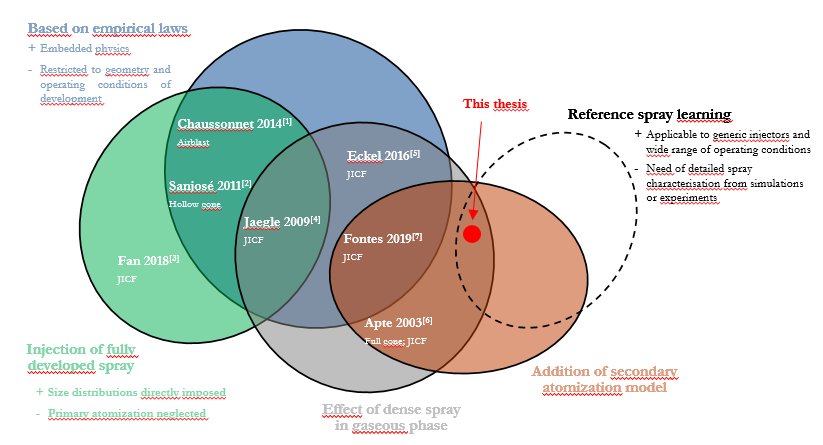
\includegraphics[scale=0.5]{./part1_numerical_approaches/figures_ch3/state_art_lagrangian}
	\caption{Classification of lagrangian injection models}
	\label{fig:state_art_injection}
\end{figure}

\subsection{Airblast spray}

Basically Chaussonnet.

\subsection{Hollow cone spray}

Basically FIMUR.

\subsection{Liquid jet in crossflow}

Aqui viene el arsenal.